\section*{Math 202a - HW5 - Dan Davison - \texttt{ddavison@berkeley.edu}}

\begin{mdframed}
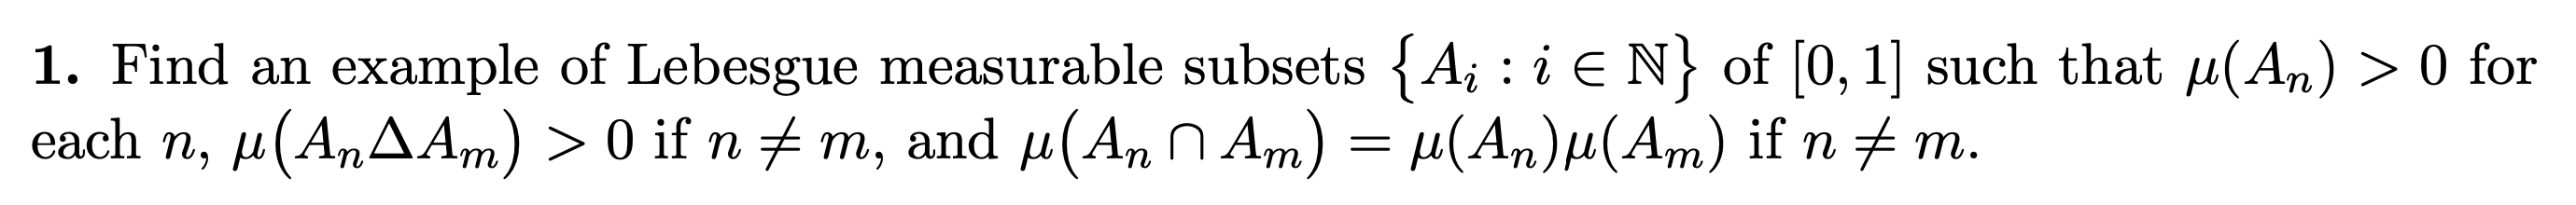
\includegraphics[width=400pt]{img/analysis--berkeley-202a-hw05-781b.png}
\end{mdframed}


\begin{definition*}
  Let $d_n(\om)$ be the $n$-th digit in the binary expansion of $\om$. If $\om$ has two equivalent binary
  expansions, we use the non-terminating one. Define
  \begin{align*}
    A_n := \{\om ~:~ d_n(\om) = 0, ~ \om \in [0, 1]\}.
  \end{align*}
  Thus, for example, $A_1 = (0, 1/2]$ and $A_2 = (0, 1/4] \cup (1/2, 3/4]$.
\end{definition*}

\begin{claim*}
  $A_n$ is Lebesgue measurable for all $n \in \N$.
\end{claim*}

\begin{proof}
  Since $A_n$ is a finite union of intervals of the form $(a, b]$, and since
  \begin{align*}
    (a, b] = \bigcap_{n=1}^\infty (a, b + n^{-1}),
  \end{align*}
  we see that $A_n$ is a finite union of open intervals in $[0, 1]$, hence in the Borel $\sigma$-algebra
  on $[0, 1]$, and hence in the Lebesgue $\sigma$-algebra on $[0, 1]$.
\end{proof}

\begin{claim*}
  $\mu(A_n) > 0$ for all $n$.
\end{claim*}

\begin{proof}
  Note that $(0, 2^{-n}] \subseteq A_n$, therefore by monotonicity of measure
  \begin{align*}
    \mu(A_n) \geq \mu((0, 2^{-n}]) = 2^{-n} > 0.
  \end{align*}
\end{proof}

\begin{claim*}
  $\mu(A_n \Delta A_m) > 0$ if $n \neq m$.
\end{claim*}

\begin{proof}
  Let $m \neq n$ and suppose without loss of generality that $m < n$.

  Then $(0, 2^{-m}] \subseteq A_m$ and also $(2^{-n}, 2^{-(n+1)}] \subset A_m$.
  But $(2^{-n}, 2^{-(n+1)}] \subset A_n^c$ and has non-zero measure, therefore $\mu(A_n \Delta A_m) > 0$.
\end{proof}

\begin{claim*}
  $\mu(A_n \cap A_m) = \mu(A_n)\mu(A_m)$ if $n \neq m$.
\end{claim*}

\begin{proof}
  Let $m \neq n$ and suppose without loss of generality that $m < n$.

  Recall that half of the rank-$i$ dyadic intervals are contained within $A_i$ (those corresponding to
  the $i$-th digit being zero). Therefore $A_i$ is the union of $2^{i-1}$ intervals each of length $2^{-i}$,
  and we have for all $i$
  \begin{align*}
     \mu(A_i) = 2^{i-1}2^{-i} =\frac{1}{2},
  \end{align*}
  therefore $\mu(A_n)\mu(A_m) = \frac{1}{4}$.

  So we need to show that $\mu(A_n \cap A_m) = \frac{1}{4}$.

  Recall that $A_m$ is the union of $2^{m-1}$ dyadic intervals. Let $I$ be one of these intervals. Recall
  that $I$ is partitioned exactly by $2^{n-m}$ rank-$n$ dyadic intervals, each of length $2^{-n}$, and that one
  half of these consist entirely of real numbers with $m$-th digit zero, while the other half have $m$-th digit
  one. Therefore,
  \begin{align*}
    \mu(A_n \cap A_m) = 2^{m-1}2^{n-m}2^{-n}2^{-1} = \frac{1}{4}.
  \end{align*}
\end{proof}
\newpage
\begin{mdframed}
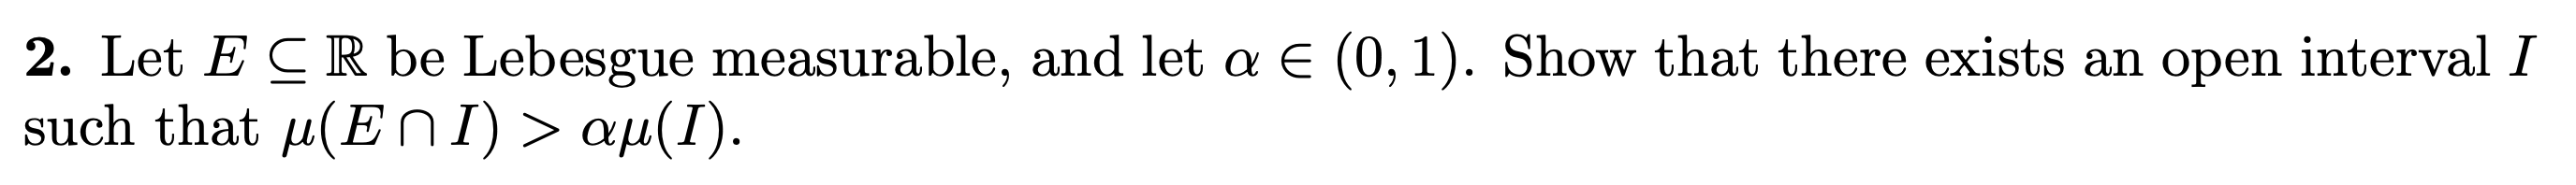
\includegraphics[width=400pt]{img/analysis--berkeley-202a-hw05-2e34.png}
It is specified also that $\mu(E) > 0$.
\end{mdframed}


\begin{proof}

\end{proof}


\newpage
\begin{mdframed}
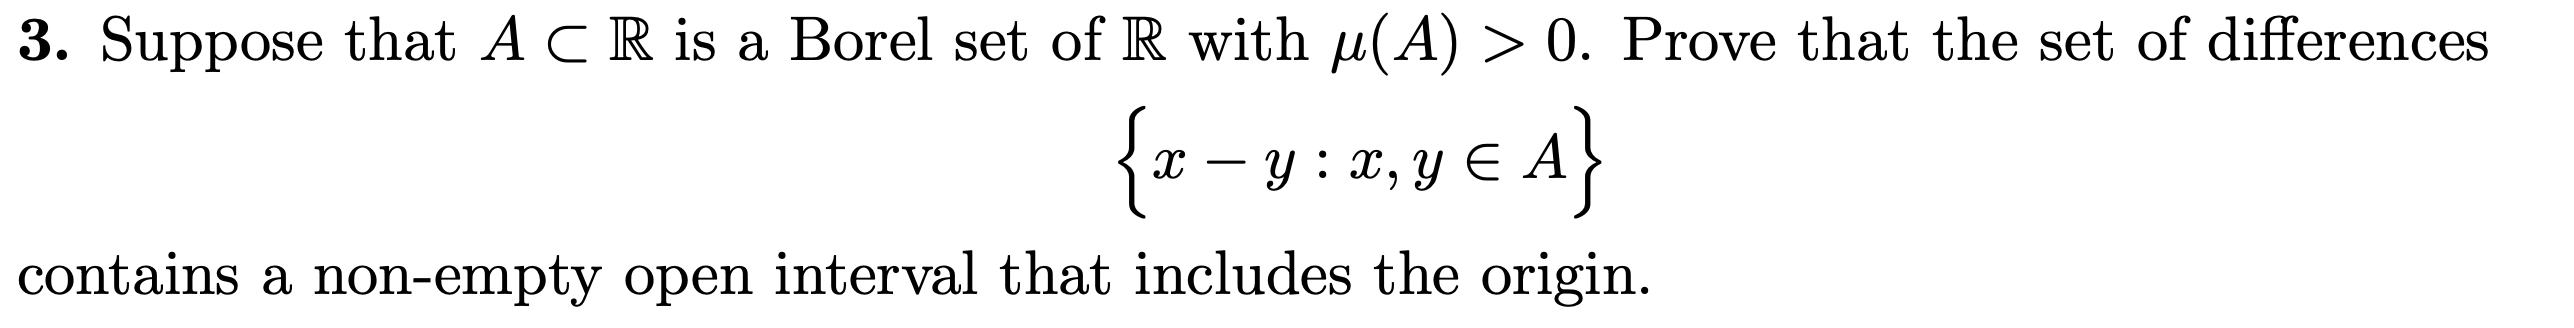
\includegraphics[width=400pt]{img/analysis--berkeley-202a-hw05-ad8b.png}
\end{mdframed}


\begin{proof}
  Now let's solve it for an example that does not contain an open interval.

  Let $A$ be a generalized Cantor set with $\mu(A) > 0$.

  let $D = \big\{ x - y ~:~ x, y \in A\big\}$.

  Since $\mu(A) > 0$ we have that $A \neq \emptyset$. Let $a \in A$. Then $a - a = 0 \in D$.

  We need to show that there exists $\epsilon > 0$ such that $(-\eps, \eps) \subseteq D$.

  We can define $z: A^2 \to (-1, 1)$. This is defined on a (complicated) closed subset of $\R^2$.

  It seems like we want to show that, within the Cantor set, there is a small region that ``behaves like​'' an
  interval, in that the image of $z$ on that region contains an open interval around the origin.
\end{proof}


\begin{proof}
  Let $A \subset \R$ be a Borel set of $\R$ with $\mu(A) > 0$.

  Let $D = \big\{ x - y ~:~ x, y \in A\big\}$.

  We need to show that there exists $\epsilon > 0$ such that $(-\eps, \eps) \subseteq D$.

  Since $\mu(A) > 0$ we have that $A \neq \emptyset$. Let $a \in A$. Then $a - a = 0 \in D$.

  We have that $\mu(A) > 0$. However, we cannot conclude that $A$ includes an interval (since $A$ could be, for
  example, the Cantor set).

  By Bass Proposition 4.14 (2) for any $\eps > 0$ there exists a closed set $G \subseteq A$ such that $\mu(A \setminus G) < \eps$.

  ... I was thinking to show that this implied the existence of an open interval included in $A$ but that's not
  true for generalized Cantor sets so it seems like that's the real problem we need to overcome.
\end{proof}


\begin{proof}
  First let's solve a simpler version.

  Let $A$ be an open set. Then $A$ contains an open interval.

  Let $B = (a, b)$ and let $D = \big\{ x - y ~:~ x, y \in A\big\}$.

  We need to show that there exists $\epsilon > 0$ such that $(-\eps, \eps) \subseteq D$.

  Intuitively this is true because we can define $z:(a, b)^2 \to (-w, w)$, where $w = b - a$. The image
  of $(a, b)^2$ under $z$ is $(-w, w)$, which contains open intervals of the desired form.
\end{proof}




\newpage
\begin{mdframed}
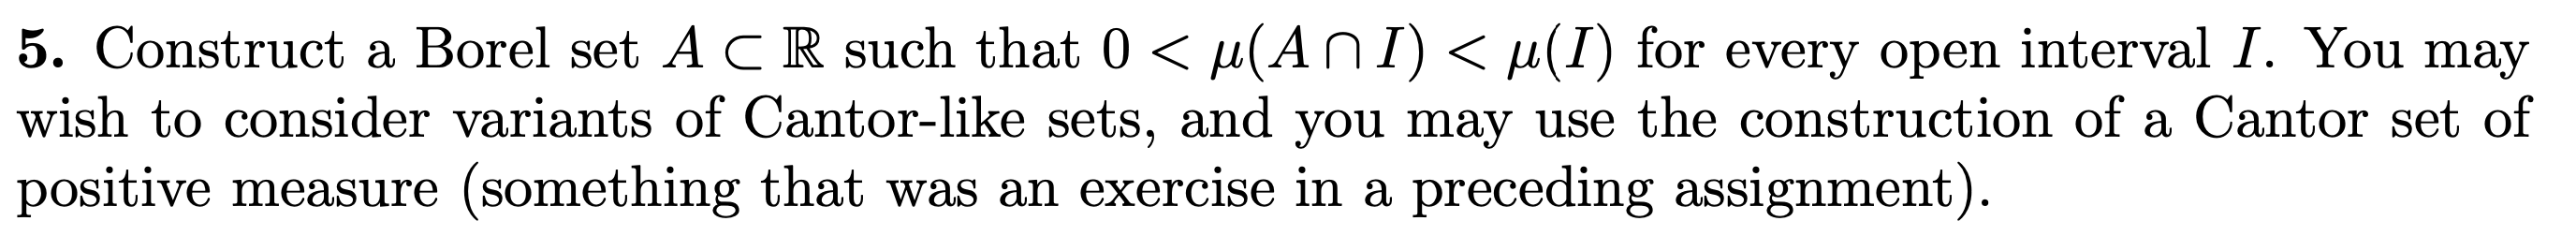
\includegraphics[width=400pt]{img/analysis--berkeley-202a-hw05-40cd.png}
\end{mdframed}

\begin{proof}
  We will use the following facts:
  \begin{enumerate}
  \item Every open interval contains a rational.
  \item A Cantor-like set includes no interval and yet has positive measure (and is uncountable).
  \end{enumerate}

  Basically what we want to do is construct $A$ from Cantor-like sets that contains every rational and yet
  includes no interval. Because $A$ includes no interval we will have $\mu(A \cap I) < \mu(I)$ for every
  interval $I$. And because $A$ is Cantor-like we will have $0 < \mu(A \cap I)$.

  Let $C: \Q \to \ms{P}(\R)$ be a function that associates with every rational a certain Cantor-like set.
  Specifically, for $q \in \Q$ we construct $C(q)$ as follows:

\end{proof}

\newpage
\begin{mdframed}
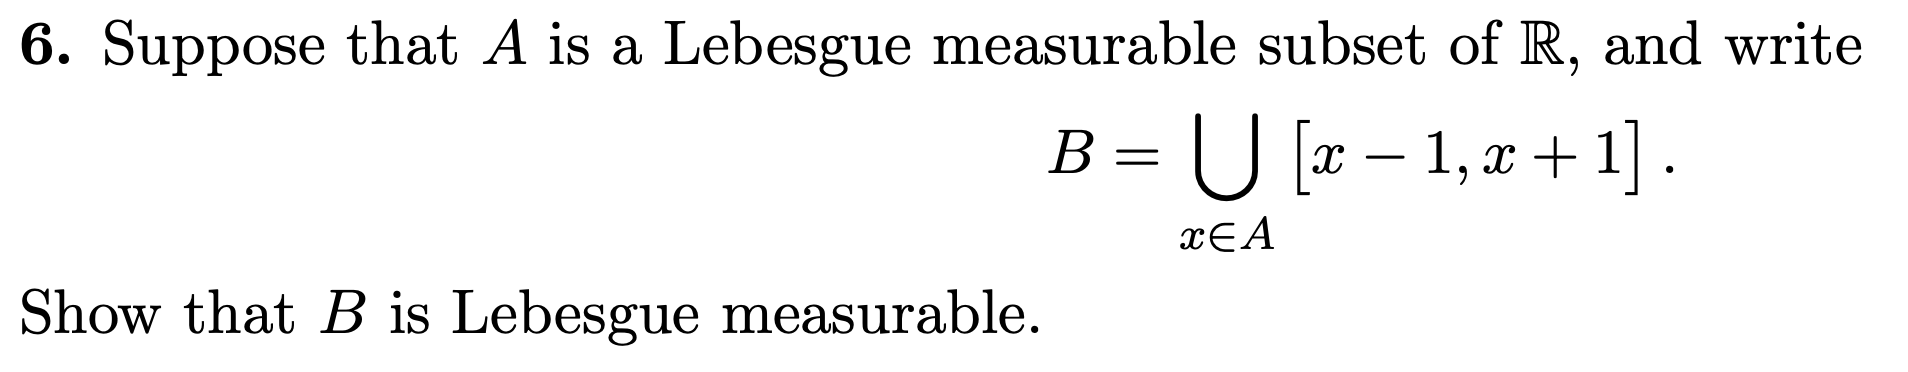
\includegraphics[width=400pt]{img/analysis--berkeley-202a-hw05-3d2c.png}
\end{mdframed}

\begin{proof}

\end{proof}